\chapter{Compiler Design}
\label{ch:compiler-design}

The compiler translates a DSL module into C sources, headers, tests, and optionally a benchmarking harness. Its stages are parsing, AST construction, type checking, IR generation, and code generation. The IR is explicit enough to control vectorization and carry placement while the source language stays compact.

\section{Pipeline Overview}
\label{sec:pipeline-overview}

The compiler takes a DSL source file, a field description, and a target description. The field description is \(\pi,\theta\), defining \(2^\pi-\theta\). The target description includes platform, vectorization mode, lane count, multiplication algorithm, unrolling factor, and delayed-realignment mode.

\paragraph{Generated artifacts.}
From these inputs it produces generated C sources and headers, which it then hands over to a C/C++ compiler (GCC or Clang) and build system (CMake, Ninja)~\cite{gcc,clang,cmake,ninja}. If requested, it also emits Boost-based correctness tests and a standalone performance harness. \Cref{fig:compiler-overview} summarizes the pipeline.

\begin{figure}[t]
    \centering
    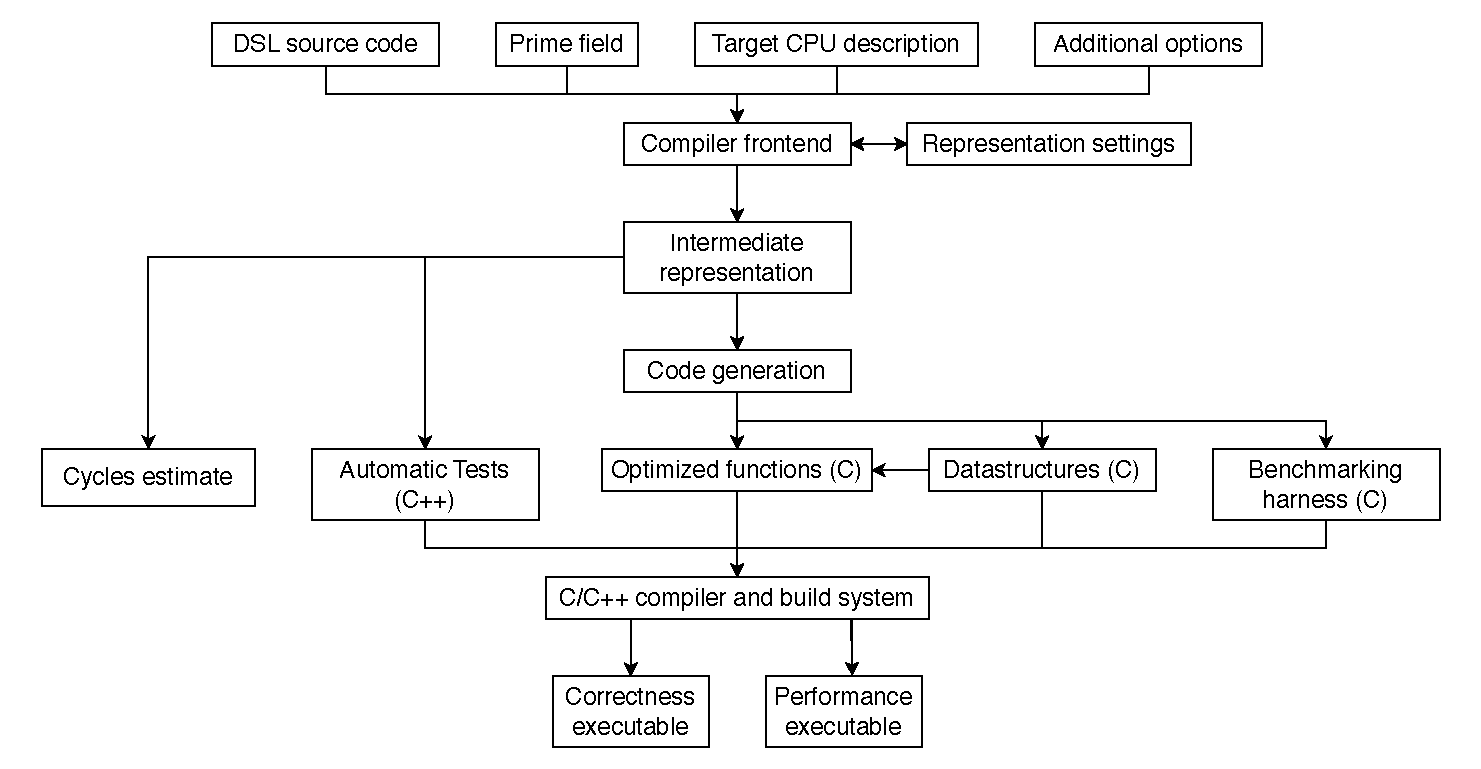
\includegraphics[width=\textwidth]{import_figures/overview.pdf}
    \caption{Overview of the compiler pipeline from DSL source, field parameters, and target description to generated C code, tests, and performance harnesses.}
    \label{fig:compiler-overview}
\end{figure}

\section{Parsing and AST Construction}
\label{sec:parsing-ast}

The concrete syntax is described by an ANTLR grammar~\cite{parr2013antlr}. ANTLR generates a Python parser; the compiler visits the parse tree and constructs an abstract syntax tree (AST).

\paragraph{AST shape.}
The AST mirrors the language rather than the grammar. It contains nodes for modules, functions, expressions, reductions, conditionals, buffer loads, literals, unary operations, and binary operations. Grammar-only details such as precedence levels disappear after parsing.

\section{Type Checking}
\label{sec:type-checking}

The type checker assigns DSL types and verifies consistent use. Index operations operate on index values; field operations on field elements; buffer loads produce field elements; reductions require bodies of the expected type. Binary arithmetic operators require equal operand types. Comparisons also require equal operand types, but produce an index value. Exponents must be index expressions and only the supported small exponents are accepted.

Hash functions must have the fixed DSL-level shape corresponding to key buffer, message buffer, and length. Helper functions may be more general, but cannot return buffers.

\section{Intermediate Representation}
\label{sec:ir}

The IR is a structured representation of the C code that will be emitted, not an assembly language.

\paragraph{Functions and mutation.}
An IR module contains functions; functions contain instructions, loops, conditionals, returns, and stores. Instructions produce or update operands. Most temporaries are SSA-like, but accumulator updates and in-place carry operations explicitly update an existing destination.

\paragraph{Instruction vocabulary.}
The instruction set includes scalar index operations, field operations, memory operations, representation-management operations, and vector helpers. Examples are \texttt{add}, \texttt{mul}, \texttt{square}, \texttt{load}, \texttt{vload}, \texttt{carry}, \texttt{vcarry}, \texttt{splat}, and \texttt{select}. Vectorized instructions are introduced by IR generation when an expression is lowered over several lanes. \Cref{app:ir-instructions} lists all instructions.

\Cref{lst:squaresum-ir} shows the pretty-printed IR for \Cref{lst:squaresum-dsl}, compiled for \(GF(2^{116}-3)\) on two-lane NEON with vectorization, schoolbook arithmetic, fully delayed limb realignment, and unrolling factor one. The sum becomes a vectorized main loop, followed by a scalar tail. Since realignment is fully delayed, the loop contains no intermediate carry instruction; \texttt{full\_reduction} appears before the store.

\begin{lstlisting}[style=thesisIR,caption={Pretty-printed IR for the vectorized square-sum running example in \(GF(2^{116}-3)\).},label={lst:squaresum-ir}]
module squaresum

hash squaresum(%key: buffer/pod, %message: buffer/pod, %len: index/scalar) -> prime<116, 3>/vector {
    %0: index/scalar = sub %len, 0
    %1: index/scalar = mod %0, 2
    %2: index/scalar = sub %len, %1
    %3: prime<116, 3>/matrix = const 0
    loop var %i from 0 to %2 step 2 {
        %4: prime<116, 3>/matrix = vload %message, %i, 0, 1
        %5: prime<116, 3>/matrix = vsquare %4
        %3 = vadd %3, %5
    }
    %6: prime<116, 3>/vector = horiz_add %3
    loop var %i from %2 to %len step 1 {
        %7: prime<116, 3>/vector = load %message, %i, 0
        %8: prime<116, 3>/vector = square %7
        %6 = add %6, %8
    }
    %6 = full_reduction %6
    store %6
}
\end{lstlisting}

\subsection{IR Types}
\label{subsec:ir-types}

The IR uses three representation types: scalar, vector, and matrix. An index value is scalar. A single field element represented by several limbs is a vector. Several field elements distributed across SIMD lanes form a matrix, because each limb component is itself a SIMD vector.

\section{Lowering Ordinary Expressions}
\label{sec:lowering-expressions}

Most expression lowering is local. Literals lower to \texttt{const}. Identifiers lower to bound parameters, loop variables, or temporaries. Buffer reads lower to \texttt{load} or \texttt{vload}, depending on requested lanes.

Unary minus becomes subtraction from zero. Binary operations lower by operand type: index operands become scalar C operators, while field operands become field instructions, vectorized when more than one lane is requested. Exponentiation is simplified: \(x^0\) becomes one, \(x^1\) becomes \(x\), and \(x^2\) becomes square.

\section{Lowering Reductions}
\label{sec:lowering-reductions}

Reductions carry most of the optimization structure and are lowered explicitly in the IR.

\paragraph{Sums.}
For sums, the compiler creates an accumulator and emits a loop over the index domain. With vectorization, the loop step is multiplied by the SIMD lane count. Each vectorized iteration evaluates several body instances in parallel; a scalar tail handles leftovers.

\paragraph{Horner reductions.}
Horner reductions are sequential in their simplest form, but can be vectorized by evaluating several branches in parallel using precomputed powers of the key. The compiler evaluates the multiplier once, constructs lane powers, and emits a vectorized loop plus scalar tail.

\paragraph{Left folds.}
Left folds are scalar loops. The accumulator is bound in the compile context for the body expression. The compiler supports unrolling, but not vectorization, because the intended use case has a loop-carried dependency.

\section{Unrolling and Carry Placement}
\label{sec:unrolling-carry}

The unrolling factor reduces loop overhead and controls carry insertion in partially delayed mode. Several logical reduction steps are emitted before a carry; the tail loop handles leftovers.

In fully delayed mode, intermediate carries are omitted and the function relies on final full reduction. Arithmetic safety depends on the field, limb representation, reduction structure, and unrolling factor.

\Cref{lst:carry-delay-schedule} shows the difference schematically.

\begin{lstlisting}[style=thesisIR,caption={Schematic carry-placement strategies for a reduction loop.},label={lst:carry-delay-schedule}]
partial:
    iter_0; iter_1; ...; iter_{u-1}; carry
    iter_u; iter_{u+1}; ...; iter_{2u-1}; carry
    ...
    full_reduction

full:
    iter_0; iter_1; iter_2; ...; iter_n
    full_reduction
\end{lstlisting}

\section{Vectorization}
\label{sec:compiler-vectorization}

Vectorization compiles selected expressions with more than one lane. The compile context records loop-index offsets, so \(message[i]\) becomes loads from \(message[i]\), \(message[i+1]\), etc., packed into a vectorized field value.

Generated temporaries use full machine width, typically 64 bits per limb. Multiplication code may narrow or mask operands internally.

\section{Conditionals}
\label{sec:compiler-conditionals}

The IR distinguishes constant-time and non-constant-time conditionals. A constant-time conditional lowers to both branches followed by a select; a non-constant-time conditional lowers to an ordinary branch.

\section{Configuration and Target Parameters}
\label{sec:configuration-targets}

The compiler configuration fixes field and machine parameters. Given \(\pi\), \(\theta\), target platform, and vectorization mode, it selects a limb arrangement. Following SPHGen~\cite{pegolotti2026sphgen}, it chooses a large limb size that reduces limb count without overflowing during configured arithmetic. It also selects multiplication algorithm, unrolling factor, and delayed-realignment mode.

\paragraph{Supported targets.}
The implementation focuses on scalar code, two-lane 64-bit ARM NEON, and four-lane 64-bit AVX2.

\paragraph{Configuration responsibility.}
The compiler exposes these choices but does not prove that every combination is safe. Aggressive unrolling or fully delayed carries can exceed available limb slack; generated tests are intended to catch such mistakes.
